\documentclass[UTF8,a4paper,11pt,fontset=none]{ctexart}
\usepackage[margin=2.1cm]{geometry}
\usepackage{fontspec,booktabs,tabularx,longtable,amsmath,amssymb}
\usepackage{graphicx,float,fancyhdr,xurl,fvextra,caption,placeins}
\usepackage[hidelinks]{hyperref}
\setmainfont{DejaVu Serif}
\setsansfont{DejaVu Sans}
\setmonofont{DejaVu Sans Mono}[Scale=0.86]
\IfFontExistsTF{Noto Serif CJK SC}{\setCJKmainfont{Noto Serif CJK SC}}{\setCJKmainfont{SimSun}[AutoFakeBold=2.5]}
\IfFontExistsTF{Noto Sans CJK SC}{\setCJKsansfont{Noto Sans CJK SC}}{\setCJKsansfont{Microsoft YaHei}}
\setCJKmonofont{Microsoft YaHei}
\ctexset{section={format=\Large\bfseries},subsection={format=\large\bfseries}}
\setcounter{tocdepth}{2}
\setlength{\parskip}{0.15em}
\linespread{1.02}
\setlength{\emergencystretch}{2em}
\renewcommand{\arraystretch}{1.22}
\raggedbottom
\pagestyle{fancy}
\fancyhf{}
\fancyhead[L]{\small 互联网数据库开发 · 个人作业 1}
\fancyhead[R]{\small 2413581 黄奕浩}
\fancyfoot[C]{\thepage}
\setlength{\headheight}{14pt}
\captionsetup{font=small,labelsep=quad}
\fvset{fontsize=\footnotesize,numbers=left,numbersep=7pt,frame=none,breaklines=true,breakanywhere=true,breakautoindent=true,tabsize=2}
\newcommand{\code}[1]{\texttt{#1}}
\hypersetup{pdftitle={Web前端初探与学习专注助手实现},pdfauthor={黄奕浩 2413581}}
\begin{document}
\begin{titlepage}
\thispagestyle{empty}\centering
\vspace*{.6cm}

\includegraphics[width=.43\textwidth]{figures/nankai_logo_color.png}
\vspace{.9cm}
\rule{.88\textwidth}{.8pt}\par\vspace{.55cm}
{\fontsize{28pt}{35pt}\selectfont\bfseries 互联网数据库开发课程实验报告\par}
\vspace{.65cm}
{\fontsize{21pt}{29pt}\selectfont\bfseries 个人作业 1\quad Web前端初探\par}
\vspace{.55cm}\rule{.88\textwidth}{.8pt}\par
\vspace{1.55cm}
{\fontsize{19pt}{28pt}\selectfont\bfseries 姓名：黄奕浩\qquad 学号：2413581\par}
\end{titlepage}
{\small\tableofcontents}
\clearpage

\FloatBarrier
\section{实验目标与环境}
\FloatBarrier
\subsection{实验环境与复现方法}
\begin{table}[H]
\centering\small
\begin{tabularx}{\textwidth}{@{}XX@{}}\toprule
项目 & 配置\\
\midrule
网页地址 & \url{http://127.0.0.1:8761}\\
服务端 & Python 3.13 标准库 http.server 与 sqlite3\\
客户端 & Microsoft Edge；jQuery 3.7.1 本地文件\\
数据 & 六项学习资源；留言写入 SQLite\\
插件 & Manifest V3；storage、activeTab、scripting、alarms 权限\\
\bottomrule\end{tabularx}
\end{table}

双击“启动实验1.cmd”，保持窗口打开，然后访问网页地址。源码目录为“网站”，服务入口为 server.py。停止时在服务窗口按 Ctrl+C。

HTTP 证据位于“请求证据”目录。browser-network.har 可通过 Edge 的 Network 面板导入。HAR 仅保留本实验网页请求，不包含 WordPress 后台登录记录。

本实验记录 HTTP 应用层报文和浏览器网络日志，展示方法、URL、请求头、请求体、响应状态和响应正文。

\FloatBarrier
\section{HTTP请求分析}
\FloatBarrier
\subsection{GET 请求与响应}
GET 在 URL 查询字符串中传入 category。服务端解析后返回两项数据库资源。此接口只读取数据。响应 Content-Type 为 JSON，状态码为 200。中文参数使用 URL 百分号编码。

\VerbatimInput{code/snippet-01.txt}

下图展示自制请求调试页的运行结果。点击按钮调用学习网页的接口，左侧显示请求方法、地址及脚本设置的请求头和请求体，右侧显示响应状态、响应头和 JSON 正文。

\begin{figure}[H]\centering
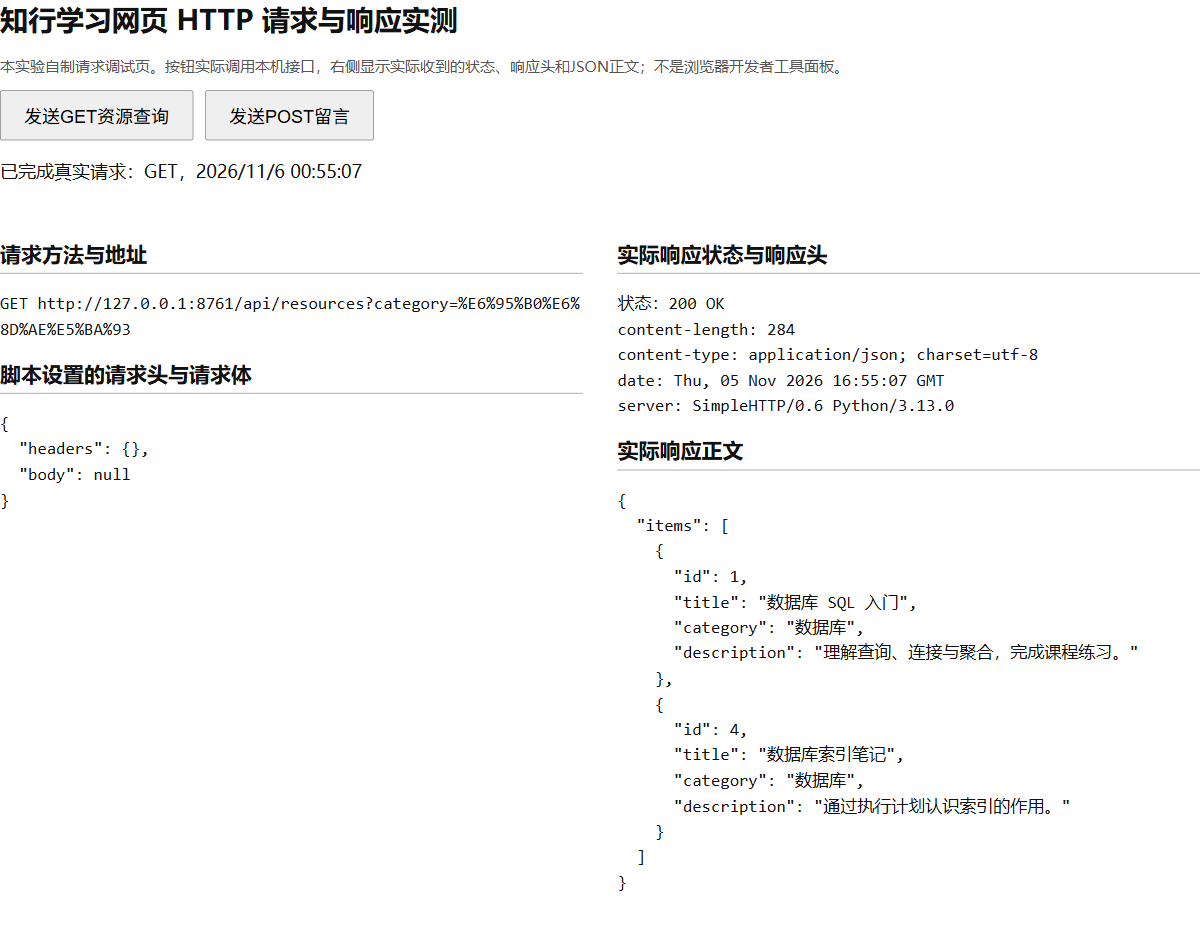
\includegraphics[width=\linewidth,height=.50\textheight,keepaspectratio]{figures/http-get.png}
\caption{GET实际请求与响应关键区域}\label{evidence:GET}
\end{figure}


\FloatBarrier
\subsection{POST 请求与响应}
POST 使用 JSON 请求体提交姓名和留言。服务端校验后使用参数化 SQL 写入 SQLite，返回 201 Created 和留言编号。前端收到响应后追加列表项。

\VerbatimInput{code/snippet-02.txt}

下图展示自制请求调试页的运行结果。点击按钮调用学习网页的接口，左侧显示请求方法、地址及脚本设置的请求头和请求体，右侧显示响应状态、响应头和 JSON 正文。

\begin{figure}[H]\centering
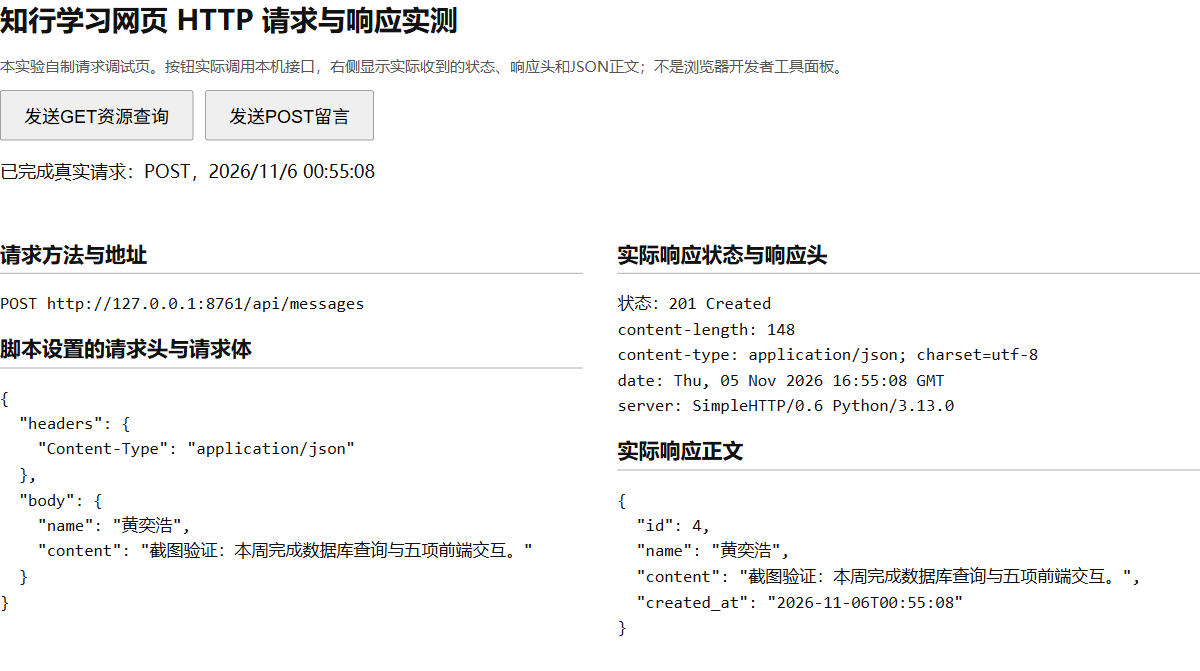
\includegraphics[width=\linewidth,height=.50\textheight,keepaspectratio]{figures/http-post.png}
\caption{POST实际请求与响应关键区域}\label{evidence:POST}
\end{figure}


\FloatBarrier
\subsection{请求比较与异常验证}
\begin{table}[H]
\centering\small
\begin{tabularx}{\textwidth}{@{}XXX@{}}\toprule
维度 & GET & POST\\
\midrule
本实验用途 & 查询资源列表 & 新建留言\\
参数位置 & URL 查询字符串 & JSON 请求体\\
数据影响 & 不修改资源 & 写入留言表\\
成功状态 & 200 OK & 201 Created\\
\bottomrule\end{tabularx}
\end{table}

POST 不会自动加密，请求体也需要 HTTPS 保护。GET 是否被缓存取决于缓存头、浏览器和中间缓存配置。重复执行本实验 POST 会增加一条留言。

补充验证：空姓名或空留言返回 400；OPTIONS 返回 204 并声明允许的方法。

\VerbatimInput{code/snippet-03.txt}

\FloatBarrier
\section{五项jQuery交互实现与验证}
\FloatBarrier
\subsection{jQuery 交互 1 搜索资源}
触发事件：input。输入 SQL 后，六项资源变为一项。搜索在已加载的数据中执行，不额外发起网络请求。

\VerbatimInput{code/snippet-04.txt}

\begin{figure}[H]
\centering
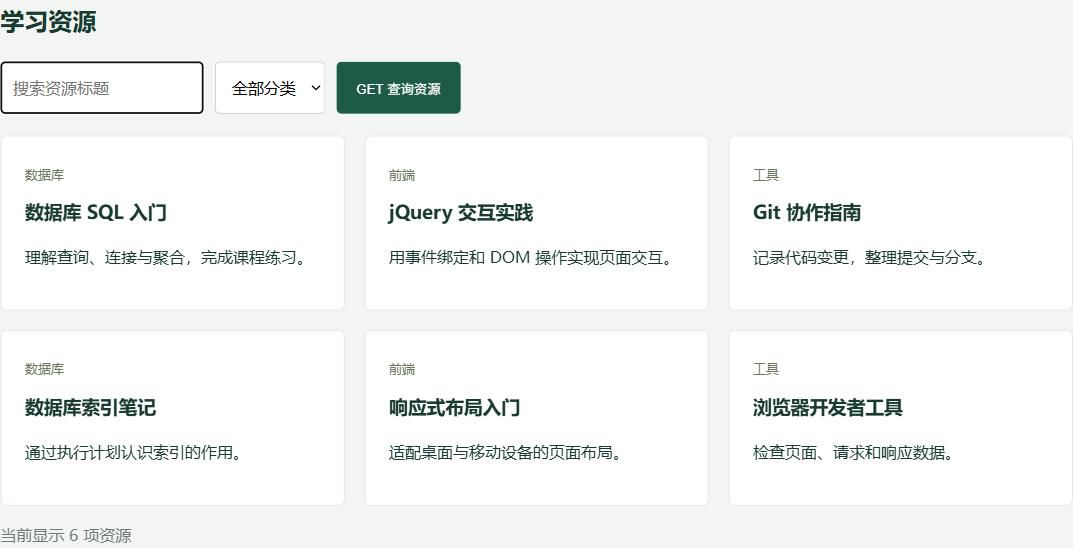
\includegraphics[width=1.0\linewidth,height=0.28\textheight,keepaspectratio]{figures/figure-01.png}
\caption{jQuery 交互 1 搜索资源 操作前}
\end{figure}

\begin{figure}[H]
\centering

\includegraphics[width=1.0\linewidth,height=0.28\textheight,keepaspectratio]{figures/figure-02.png}
\caption{jQuery 交互 1 搜索资源 操作后}
\end{figure}

\FloatBarrier
\subsection{jQuery 交互 2 分类筛选}
触发事件：change。选择前端分类后显示两项。搜索词与分类条件同时参与过滤。

\VerbatimInput{code/snippet-05.txt}

\begin{figure}[H]
\centering
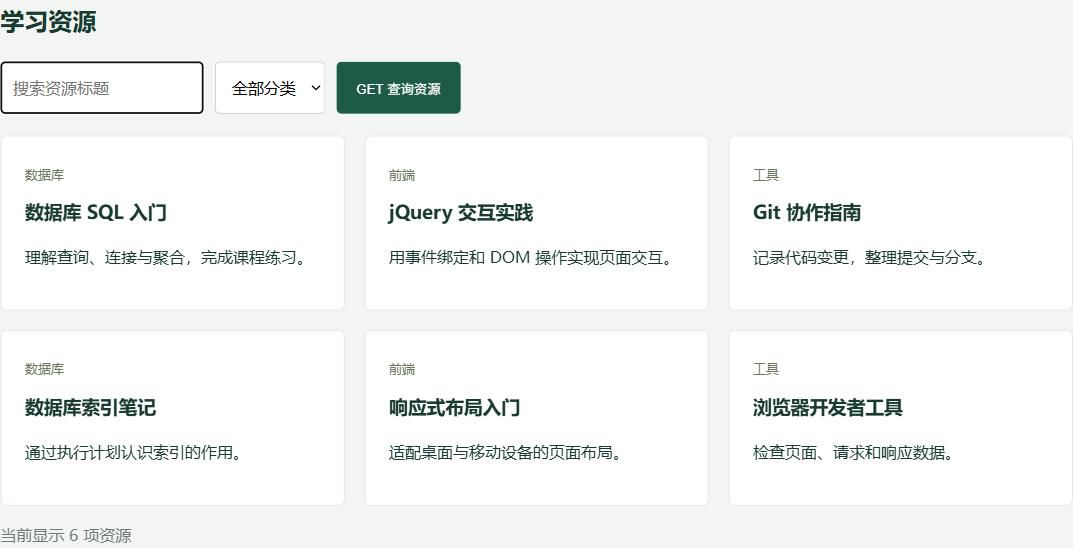
\includegraphics[width=1.0\linewidth,height=0.28\textheight,keepaspectratio]{figures/figure-03.png}
\caption{jQuery 交互 2 分类筛选 操作前}
\end{figure}

\begin{figure}[H]
\centering

\includegraphics[width=1.0\linewidth,height=0.28\textheight,keepaspectratio]{figures/figure-04.png}
\caption{jQuery 交互 2 分类筛选 操作后}
\end{figure}

\FloatBarrier
\subsection{jQuery 交互 3 展开成员}
触发事件：click。点击按钮后显示成员介绍，再次点击收起；完整源码同步更新按钮文字和 aria-expanded。

\VerbatimInput{code/snippet-06.txt}

\begin{figure}[H]
\centering

\includegraphics[width=1.0\linewidth,height=0.28\textheight,keepaspectratio]{figures/figure-05.png}
\caption{jQuery 交互 3 展开成员 操作前}
\end{figure}

\begin{figure}[H]
\centering

\includegraphics[width=1.0\linewidth,height=0.28\textheight,keepaspectratio]{figures/figure-06.png}
\caption{jQuery 交互 3 展开成员 操作后}
\end{figure}

\FloatBarrier
\subsection{jQuery 交互 4 切换主题}
触发事件：click。点击主题按钮后，页面背景、资源卡片和正文颜色变化，再次点击恢复。

\VerbatimInput{code/snippet-07.txt}

\begin{figure}[H]
\centering

\includegraphics[width=1.0\linewidth,height=0.28\textheight,keepaspectratio]{figures/figure-07.png}
\caption{jQuery 交互 4 切换主题 操作前}
\end{figure}

\begin{figure}[H]
\centering

\includegraphics[width=1.0\linewidth,height=0.28\textheight,keepaspectratio]{figures/figure-08.png}
\caption{jQuery 交互 4 切换主题 操作后}
\end{figure}

\FloatBarrier
\subsection{jQuery 交互 5 提交留言}
触发事件：submit。填写内容后提交，服务端返回 201；页面出现成功反馈并追加留言，输入框清空。

\VerbatimInput{code/snippet-08.txt}

\begin{figure}[H]
\centering
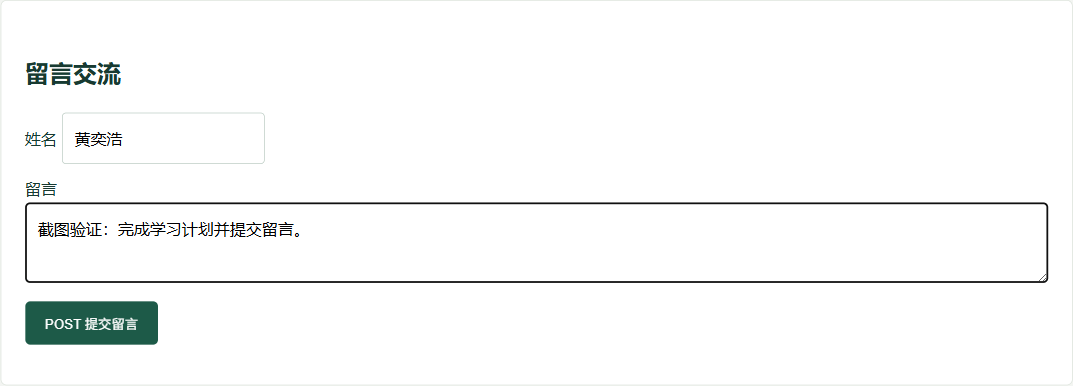
\includegraphics[width=1.0\linewidth,height=0.28\textheight,keepaspectratio]{figures/figure-09.png}
\caption{jQuery 交互 5 提交留言 操作前}
\end{figure}

\begin{figure}[H]
\centering
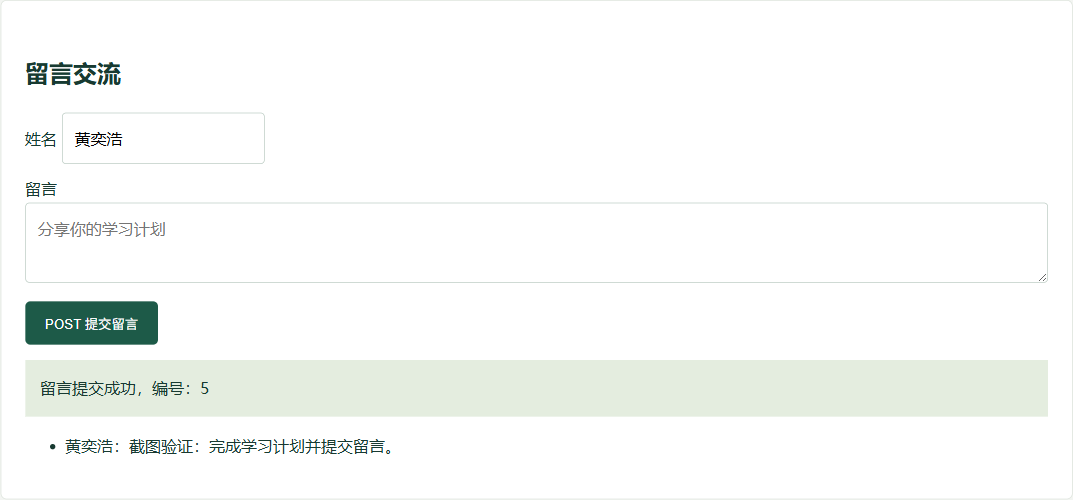
\includegraphics[width=1.0\linewidth,height=0.28\textheight,keepaspectratio]{figures/figure-10.png}
\caption{jQuery 交互 5 提交留言 操作后}
\end{figure}

\FloatBarrier
\section{浏览器插件设计与验证}
\FloatBarrier
\subsection{浏览器插件功能与安装}
知行学习专注助手提供阅读模式、1至120分钟专注计时、按网页保存本地笔记，以及 JSON 笔记导出。计时结束由后台 alarms 事件更新工具栏徽标，关闭弹出面板不会重置结束时间。

\begin{table}[H]
\centering\small
\begin{tabularx}{\textwidth}{@{}XX@{}}\toprule
权限 & 使用原因\\
\midrule
storage & 保存计时结束时间与各网页笔记\\
activeTab & 用户主动点击插件后访问当前标签页\\
scripting & 向当前普通网页注入或移除阅读模式样式\\
alarms & 关闭弹出面板后仍可触发计时结束事件\\
\url{http://127.0.0.1/*} & 访问本机实验页以验证阅读模式，不授予其他站点常驻访问\\
\bottomrule\end{tabularx}
\end{table}

插件不申请所有站点的常驻访问权限，不向外部服务器上传笔记。浏览器内部页面和扩展页面禁止脚本注入时，会显示提示；请在普通网页中使用阅读模式。

安装：打开 edge://extensions，开启开发人员模式，点击“加载解压缩的扩展”，选择“浏览器插件”文件夹。固定工具栏图标后，打开实验网页并点击插件。Chrome 的入口为 chrome://extensions。

\FloatBarrier
\subsection{插件实际运行}
\begin{figure}[H]
\centering
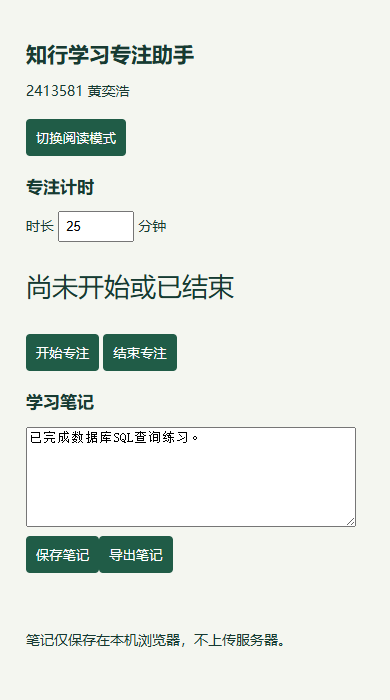
\includegraphics[width=0.52\linewidth,height=0.28\textheight,keepaspectratio]{figures/figure-11.png}
\caption{独立 Edge 扩展环境中的真实扩展页面}
\end{figure}

\begin{figure}[H]
\centering
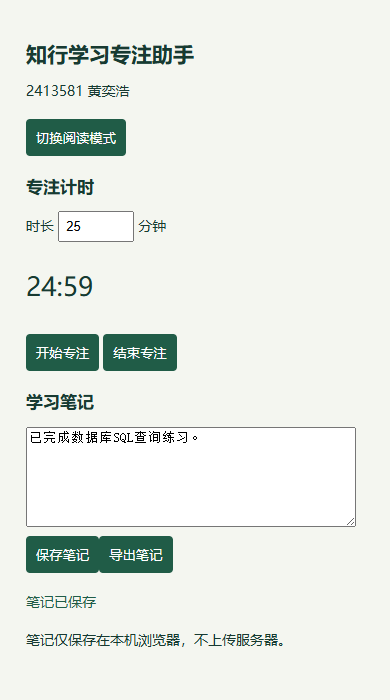
\includegraphics[width=0.52\linewidth,height=0.28\textheight,keepaspectratio]{figures/figure-12.png}
\caption{开始计时并保存学习笔记后的状态}
\end{figure}

扩展加载后可以开始和结束计时；笔记保存后，重新打开页面仍能恢复内容。图中展示扩展页面及计时、笔记保存后的状态。

\FloatBarrier
\subsection{插件阅读模式验证}
\begin{figure}[H]
\centering
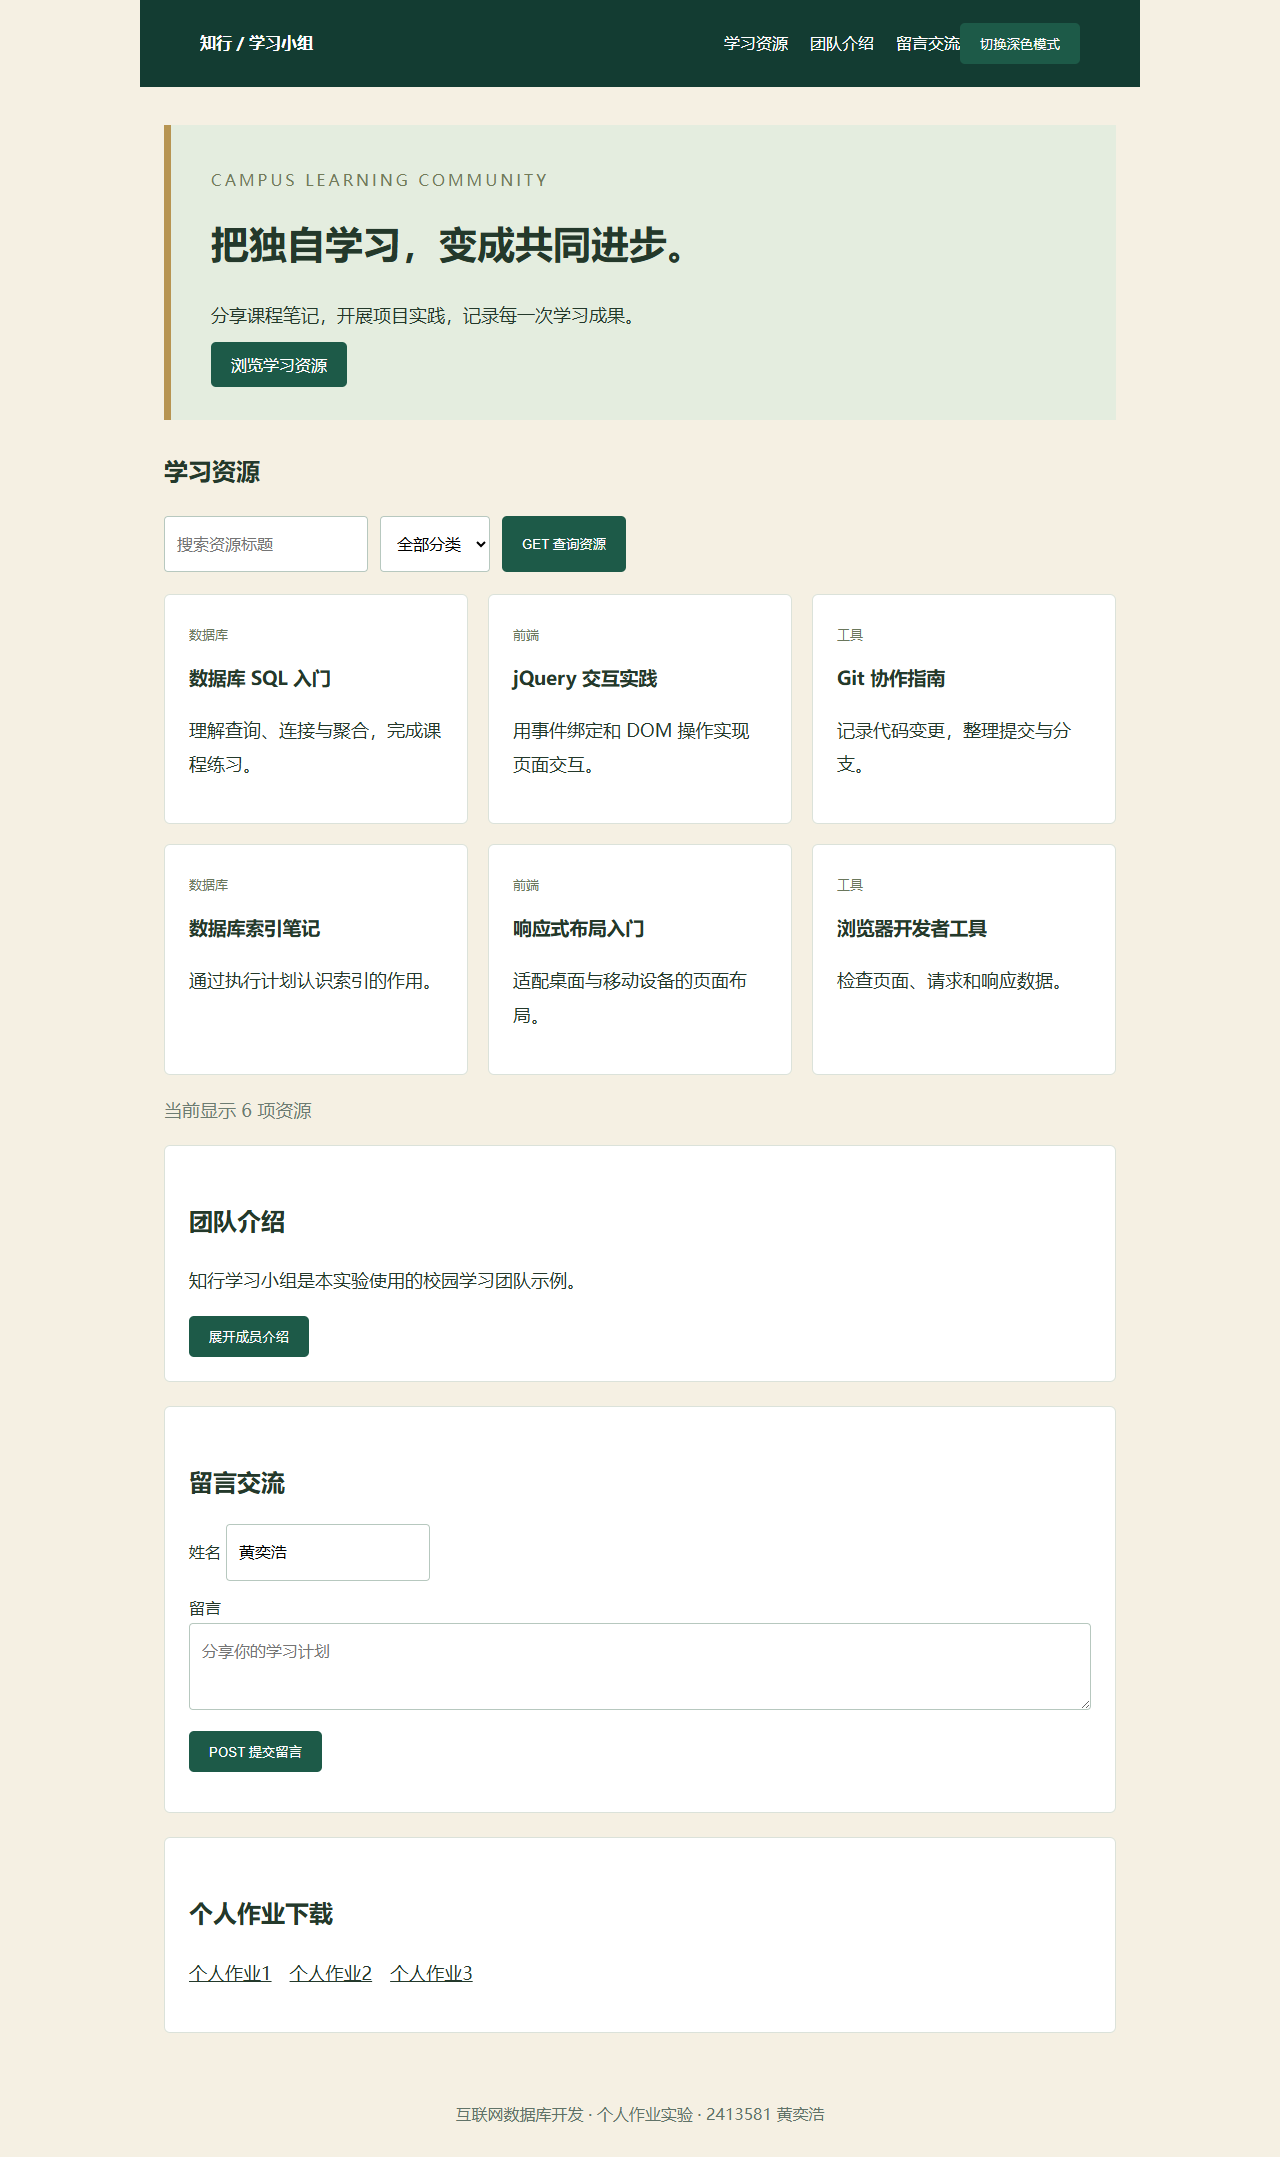
\includegraphics[width=1.0\linewidth,height=0.65\textheight,keepaspectratio]{figures/figure-13.png}
\caption{在普通实验网页中注入阅读样式后的真实效果}
\end{figure}

阅读模式将正文限制在约1000像素宽度，调整页面背景与行距，并隐藏 video 和 iframe。再次切换时移除注入的样式，恢复原页面显示。

\FloatBarrier
\section{实验结果与讨论}
\FloatBarrier
\subsection{实验结果}
搜索、分类筛选、成员展开、主题切换和留言提交均能产生相应的页面变化。GET 返回资源数据，POST 返回留言编号，空留言被服务端拒绝。用户输入通过 text() 显示，数据库写入使用参数化 SQL。

留言数据保存在本地 SQLite 数据库中，页面列表追加当前提交内容，历史留言可通过 GET /api/messages 查询。

参考资料：jQuery \url{https://api.jquery.com/} ；Chrome Extensions \url{https://developer.chrome.com/docs/extensions/reference/} ；Python http.server \url{https://docs.python.org/3/library/http.server.html} 。

\FloatBarrier\appendix
\section{源程序}
\subsection{网站/app.js}
\VerbatimInput{code/source-01.js}

\subsection{浏览器插件/manifest.json}
\VerbatimInput{code/source-02.json}

\subsection{浏览器插件/popup.html}
\VerbatimInput{code/source-03.html}

\subsection{浏览器插件/popup.css}
\VerbatimInput{code/source-04.css}

\subsection{浏览器插件/popup.js}
\VerbatimInput{code/source-05.js}

\subsection{浏览器插件/background.js}
\VerbatimInput{code/source-06.js}

\end{document}
